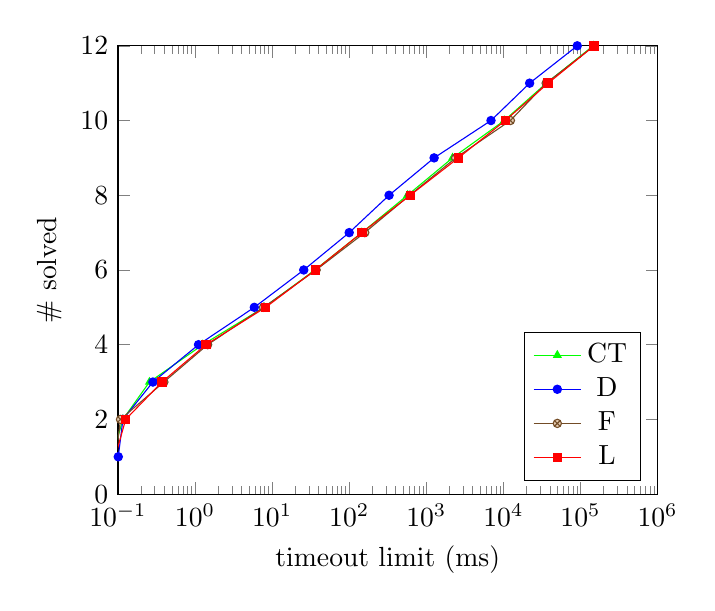
\begin{tikzpicture}[scale=1.0]
  \begin{axis}[
    xmode=log,
    ymin=0,ymax=12,
    xmin=0.1, xmax=1000000,
    every axis plot/.style={thin},
    xlabel={timeout limit (ms)},
    ylabel={\# solved},
    legend pos=south east
    % table/create on use/cumulative distribution/.style={
    %   create col/expr={\pgfmathaccuma + \thisrow{f(x)}}   
    % }
    ]
    \addplot 
    [mark=triangle*,
    mark size=1.5,
    mark options={solid},
    green] 
    coordinates {(0.084, 1)
(0.116, 2)
(0.256, 3)
(1.260, 4)
(7.875, 5)
(35.914, 6)
(145.718, 7)
(569.755, 8)
(2188.949, 9)
(10255.624, 10)
(36100.351, 11)
(146369.977, 12)};

    \addplot 
    [blue,
    mark=*,
    mark size=1.5,
    mark options={solid}]
    coordinates {(0.101, 1)
(0.116, 2)
(0.284, 3)
(1.109, 4)
(5.877, 5)
(25.704, 6)
(99.958, 7)
(328.802, 8)
(1261.949, 9)
(6902.817, 10)
(21882.579, 11)
(90746.729, 12)};

    \addplot [brown!60!black,
    mark options={fill=brown!40},
    mark=otimes*,
    mark size=1.5]
    coordinates {(0.094, 1)
(0.108, 2)
(0.394, 3)
(1.456, 4)
(7.739, 5)
(37.198, 6)
(159.031, 7)
(608.126, 8)
(2403.445, 9)
(12314.402, 10)
(35864.647, 11)
(150557.351, 12)};

    \addplot 
    [red,
    mark size=1.5,
    mark=square*]
    coordinates {(0.092, 1)
(0.126, 2)
(0.372, 3)
(1.385, 4)
(8.248, 5)
(36.259, 6)
(145.918, 7)
(618.144, 8)
(2604.808, 9)
(10555.311, 10)
(38059.606, 11)
(149972.461, 12)};
    \legend{CT,D,F,L}
  \end{axis}
\end{tikzpicture}
